% =============================================================================
%  REAL-LIFE CASE STUDY — first draft (2026-08-13)
%
%  Data:    data/Trip_Report_PD74720_2025-09-22_2025-09-27.xlsx  (not shipped;
%           carrier-confidential telematics export)
%  Build:   src/instance_gen/route_from_data.py   (route + customers + ferry)
%           src/instance_gen/osm_overlay.py       (charger and layby sets)
%           src/instance_gen/trip_vs_hypothesis.py(assumption validation)
%  Outputs: data_output/real_route_{stops,cs_hgv,cs_alternatives,restareas}.csv
%           figures/real_route_instance.png
%
%  Conventions:  plain text = number verified against a stored result file
%                \red{...}  = still pending a run, or a decision for you
%
%  ANONYMISATION: no carrier, customer, site or city name appears in this
%  section or in figures/real_route_instance.png (customers are C1--C7).
%  Country and region only.  The charging sites are public infrastructure and
%  are named only in the replication files, not here.
% =============================================================================

\subsection{Real-life case study}
\label{sec:casestudy}

The synthetic corridors of Section~\ref{sec:basecase} are generated from
distributions we control, so they cannot tell us whether the instance class
itself is realistic.  To test that, we reconstruct one instance directly from
operational data: a complete international tour driven by a Norwegian haulier
in September~2025, recorded by the vehicle's own telematics system.  The
export covers six consecutive days of a single 40\,t tractor--semitrailer at
one-minute resolution, and contains the GPS trace, the odometer, per-stop
arrival and departure times, the freight order register, and fuel and gross
weight readings.  Carrier, customers and sites are anonymised throughout; we
report country and region only.

\paragraph{Route reconstruction.}
The tour is a closed round trip from a depot in southern Norway: two
deliveries in the same region, a sea crossing to northern Denmark, then south
through Denmark and Germany to the central Netherlands, east into
north-eastern Bavaria, and back along the reverse corridor to the depot.  We
do not reconstruct the road geometry from a routing service: the vehicle
records it.  The stop sequence and the odometer distance between consecutive
stops give the arc lengths directly, and cumulative distance unrolls the tour
onto the linear stop axis $\mathcal I = \{0,\dots,N\}$ of
Section~\ref{sec:model}, with the depot at both ends.  Total length is
$3\,339$\,km.  Nominal leg travel times are set from the speeds observed on
that leg rather than from a single corridor-wide speed, since the tour mixes
Norwegian regional roads (42--66\,km/h leg averages) with German and Danish
motorway (74--85\,km/h); the realised week is retained separately as the
uncertainty realisation against which the plans are evaluated.

Customers are identified by matching stop addresses against the freight order
register, which distinguishes a load or unload operation from a driver break
at a service area.  Seven customer stops result, at km 8, 66, 1\,183, 1\,321,
1\,991, 2\,072 and 2\,117.  Their service times are the observed dwells,
ranging from 0.5\,h to 2.0\,h with a mean of 1.2\,h.  The stops the driver made
for breaks and rests are \emph{not} carried into the instance: when to stop,
and for how long, is what the model decides.

\paragraph{Sea crossing.}
The tour includes a ferry crossing in each direction, which is a feature no
synthetic instance has and which the formulation of Section~\ref{sec:model}
represents without modification.  Each crossing --- embarkation port, sailing,
disembarkation port --- is collapsed into a single layby node at which we fix
$x^{b45}_i = 1$ and $\tau^b_i = T^{\text{cross}}$.  Fixing the break binary,
rather than offering the stop as an option, is what makes the crossing
mandatory; the manoeuvre time $M^{\text{lay}}_i$ then carries the boarding and
disembarking overhead and cannot be avoided either.  Three consequences follow
from the existing constraints with no new machinery.  The crossing is dwell at
a node, so it never enters the driving accumulators $cd$ and $sd$ and is not
charged against the driving limits; it is break time, not work, so it does not
enter the working-time accumulator $sw$; and because the reset indicator
already includes $x^{b45}$, the continuous-driving clock is reset on
disembarkation.  This last point is not a modelling convenience but a
requirement.  Under Art.~9 of Regulation~(EC) No.~561/2006 a ferry
interruption counts toward the break, and the observed schedule places a drive
of nearly $4.5$\,h immediately after landing --- legal only on a reset clock.  The
crossings are fixed at their measured port-to-port durations, $3.8$\,h and
$4.9$\,h, and consume no energy.  We do not model the sailing timetable: the
crossing is available on arrival, and the waiting the driver actually did is
absorbed into the measured durations.

\paragraph{Charging and rest infrastructure.}
Neither charger nor rest-area locations can come from the trip data, since the
vehicle is diesel.  We take both from OpenStreetMap, projected onto the
reconstructed corridor.  Rest areas are the \texttt{highway=rest\_area} and
\texttt{highway=services} features within 500\,m of the trace; sites less than
5\,km apart are represented by a single node, giving $|\mathcal L| = 63$
laybys.  As a check on this set, every service area at which the driver
actually stopped appears in it.

For charging stations we admit only sites that are asserted to be
heavy-vehicle accessible (\texttt{hgv=yes} or \texttt{truck=yes}), which is far
more restrictive than filtering on rated power: of the more than $4\,500$
charging stations mapped within 3\,km of the corridor, only 18 carry such a
tag.  Widening the corridor band does not repair this, and the sweep is itself
informative --- beyond a 20\,km band the coverage stops improving, because the
gaps are gaps in \emph{tagging} and in genuine heavy-duty deployment, not an
artefact of a narrow search.  We therefore admit a site when it is
heavy-vehicle tagged, when its operator is a heavy-duty charging network, or
when its name identifies it as a truck facility, and we add three publicly
documented truck charging parks on the German section that OpenStreetMap has
not yet tagged (two of them share one motorway junction and enter as a single
node; sources are listed in the replication files).
The result is $|\mathcal K| = 43$ charging nodes, with rated powers from 150 to
1\,400\,kW (median 400\,kW); the four sites without a power tag are assigned
the base rating of Table~\ref{tab:params}.  The largest interval without a
charging node is 293\,km, which the base 500\,kWh pack covers, so the instance
is feasible at the same battery and charging parameters as the synthetic
study, with no relaxation.

A charging station off the carriageway costs the driver a detour.  We charge
this as manoeuvre time only, at
$M^{\text{stop}} + 2\max\{0,\, d_i - \bar d\}/v$, where $d_i$ is the site's
distance from the route, $v = 80$\,km/h, and $\bar d = 0.37$\,km is the mean
off-route distance of the service areas the driver used in the recorded week.
Subtracting $\bar d$ is what makes the penalty a \emph{detour}: stopping
always requires leaving the road, and only the excess over a normal stop is
attributable to the charger.  Manoeuvre times range from 0.17\,h to 0.63\,h
(median 0.24\,h).  The detour distance is not charged against the battery, which
makes the energy side of a distant charger mildly optimistic.

\paragraph{Instance class and time windows.}
Table~\ref{tab:casestudy} summarises the instance.  With $3\,339$\,km and seven
customers it falls in the Long route class ($3\,000$--$4\,000$\,km) and at the
lower edge of the Many customer class ($7$--$15$) of
Table~\ref{tab:instances}, and it spans five duty cycles, exactly the regime
that class was designed to represent; the case study therefore reads against
the Long/Many rows of Table~\ref{tab:gap} rather than as an isolated instance.
It differs from its synthetic counterparts in one telling respect.  A Long
synthetic instance carries about 167 stops, this one 117, even though the
routes are the same length: the synthetic generator places charging stations
every 60\,km, the spacing that Regulation~(EU) 2023/1804 mandates on the
core network by 2030, whereas the corridor as it exists today offers 43
heavy-vehicle sites unevenly distributed along $3\,339$\,km.  The real instance
is thus not a smaller problem but a sparser one, with fewer and less evenly
placed opportunities to charge.

We assign no customer time windows.  The delivery appointments are not part of
the telematics export, and inventing windows around the observed arrivals
would build the realised schedule into the instance and flatter every method
that reproduces it.  The case study is therefore an instance of the
\emph{None} window class, and comparisons are drawn against the Long/Many/None
row.  This is a limitation of the data, not a modelling choice: the tour was
certainly driven against delivery appointments.

\begin{table}[htbp]
\centering
\caption{The real-life instance.  Distances and times are measured from the
telematics export; charging and rest infrastructure is from OpenStreetMap with
documented additions.  Battery, charging curve, ECR and hours-of-service
parameters are unchanged from Table~\ref{tab:params}.}
\label{tab:casestudy}
\begin{tabular}{ll}
\toprule
\textbf{Quantity} & \textbf{Value} \\
\midrule
Route length                       & $3\,339$\,km, closed tour \\
Duration of the recorded week      & 6 days, 5 daily rests \\
Stops $|\mathcal I|$               & 117 \\
Customers $|\mathcal C|$           & 7 (service $0.5$--$2.0$\,h, mean $1.2$\,h) \\
Charging nodes $|\mathcal K|$      & 43 (150--1\,400\,kW, median 400\,kW) \\
Laybys $|\mathcal L|$              & 63 \\
Ferry nodes                        & 2 (forced break, $3.8$\,h and $4.9$\,h) \\
Largest gap between chargers       & 293\,km \\
Manoeuvre time at chargers         & $0.17$--$0.63$\,h (median $0.24$\,h) \\
Instance class                     & Long / Many / None \\
\bottomrule
\end{tabular}
\end{table}

\begin{figure}[htbp]
    \centering
    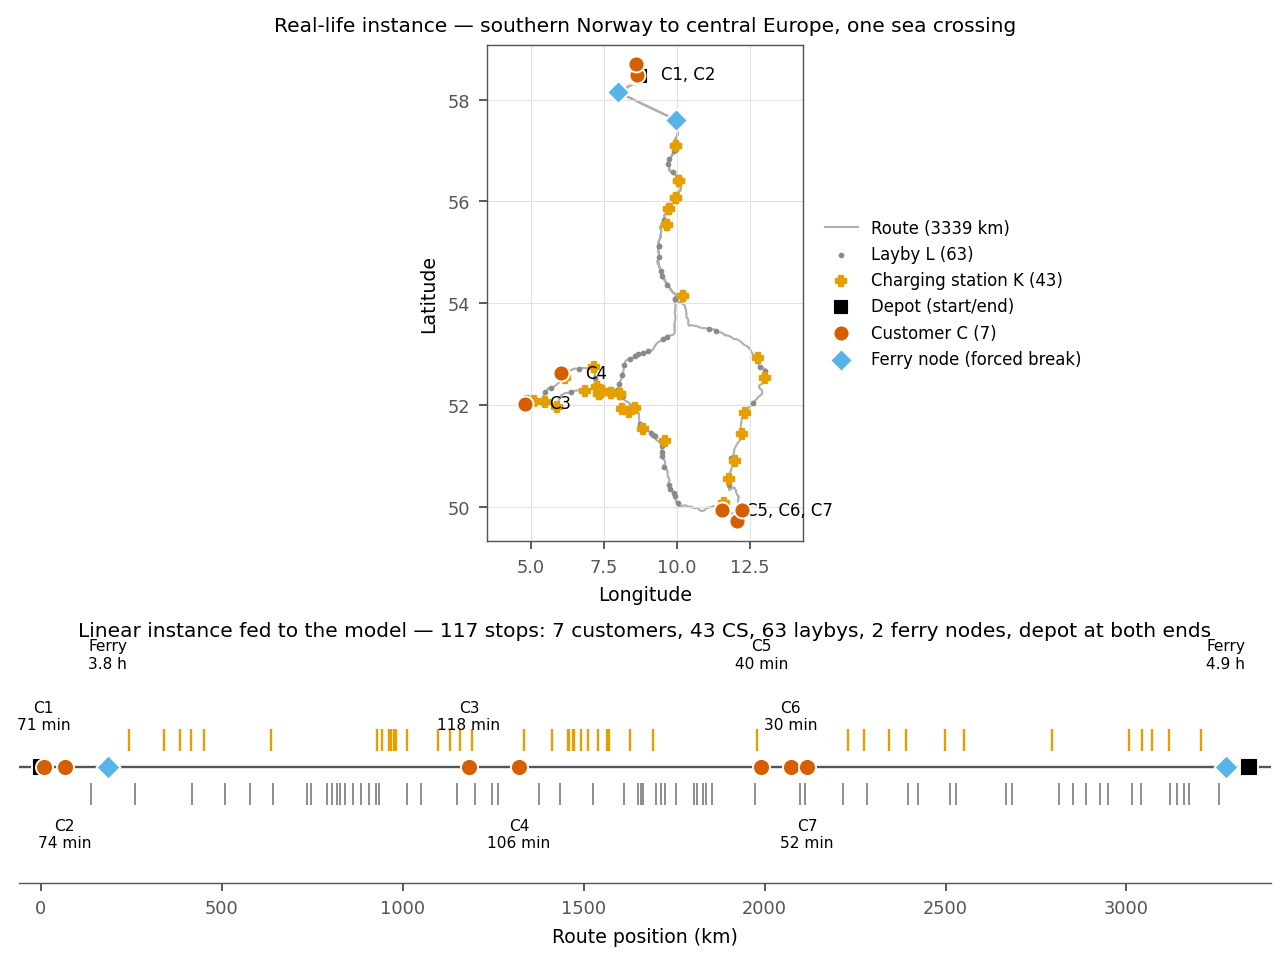
\includegraphics[width=\linewidth]{figures/real_route_instance.png}
    \caption{The real-life instance.  Top: the reconstructed corridor with the
    charging set $\mathcal K$, the layby set $\mathcal L$, the seven customers
    (anonymised as C1--C7) and the two ferry nodes.  Bottom: the same instance
    on the linear stop axis given to the model, chargers above the axis and
    laybys below.  The sea crossings add no distance, which is why the two
    ferry nodes sit at km 185 and km 3\,274 with the tour's two Norwegian
    customers and its depot on the same short segment of the axis.}
    \label{fig:caseinstance}
\end{figure}

\paragraph{The recorded schedule as a check on the model's assumptions.}
Because the export records what the driver actually did, it also lets us test
assumptions that the synthetic study can only assert.  Three hold well.  The
driver's non-customer dwells cluster at the two durations the regulation
defines, near 45\,min and near 15\,min, which is the split-break structure of
Section~\ref{sec:model}; the longest uninterrupted driving spell in the week is
$4.52$\,h against the $4.5$\,h limit, so the continuous-driving constraint is
binding in practice and not merely present; and two of the daily rests are
taken at $9.00$ and $9.03$\,h, i.e. the reduced rest is used at exactly its
legal minimum, which supports modelling reduced rests as a decision rather than
an exception.  Fuel consumption over the week, $27.4$\,L/100\,km, corresponds to
about $1.15$\,kWh/km at the wheel, against the $1.23$\,kWh/km our ECR model
gives at 80\,km/h; the difference is consistent with the recorded mean gross
weight of $25$\,t against the $40$\,t design point, so the energy model is
conservative rather than wrong.  Two assumptions are contradicted.  Service
time averages $1.2$\,h rather than the $0.5$\,h assumed in the synthetic
instances, and the nominal speed of $80$\,km/h holds on motorway legs but
overstates regional legs by a wide margin --- which is why leg times in this
instance are set per leg.

\paragraph{Results.}
\red{Pending: run all methods on the instance and report realised duration,
gap to the oracle, and infeasibility against the Long/Many/None row of
Table~\ref{tab:gap}.  Report also whether the oracle certifies within its 2\,h
budget at $|\mathcal I| = 117$, and whether the sparser and more unevenly
spaced charging set makes the methods diverge more or less than on the
synthetic Long instances.}

\paragraph{Limitations.}
Four caveats bound what the case study establishes.  The charging network is a
2026 snapshot while the tour was driven in 2025, so the instance asks how this
tour would be operated on today's infrastructure, not how it could have been
operated then.  The corridor crosses terrain with sustained gradients,
particularly on the Norwegian section, which a constant-ECR model does not
capture; on a closed tour the elevation gain nets out, but the per-leg energy
does not.  The uncertainty distribution is unchanged from the synthetic study:
one week yields one realisation, which is enough to evaluate a plan but not to
calibrate a coefficient of variation, and re-estimating it would require the
same tour repeated over many weeks.  Finally, the customer set is small
relative to the route length --- seven deliveries over $3\,339$\,km, with a
$1\,150$\,km customer-free return --- so the instance stresses the
charging and hours-of-service interaction far more than the time-window
interaction.
